In the following subsections we will describe different strategies for data set manipulation from the most naive approach to more refined approaches such as trimming and analysis. These approaches are applied to the data before sending the input to the network. These strategies are used in experiments with the actual networks to locate the best possible strategy.

\subsection{Normalization}
For artificial neural networks to do the best work; the data should be normalized to either bipolar data(-1 to 1) or binary data(0 to 1). This ensures the best performance by the activation functions since the sigmoid activation function input/output approximately follows table ~\ref{fig:same_hour_distribution}
\begin{figure}[!ht]
\centering
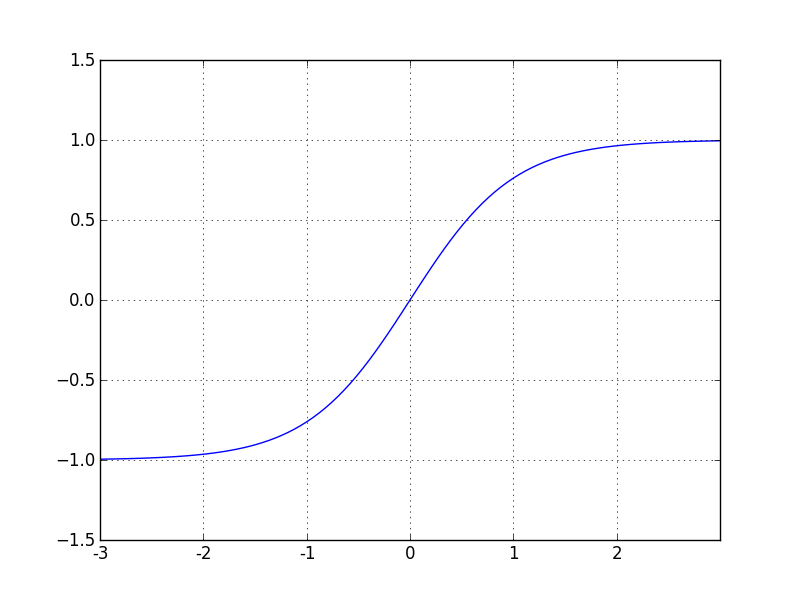
\includegraphics[width=0.8\linewidth,natwidth=898,natheight=587]{billeder/activationFunctions/tanh.png}
\caption{A simple neural network with 3 layers. \cite{stockForecasting}}
\label{fig:ANN}
\end{figure}

\subsection{The naive approach}

\subsection{Trimming}

\subsection{Matrix}

\subsection{Historical data}